\section{Analisis Spektrum Eksperimen dan Validasi Model Simulasi Fisika Maju}
\label{sec:analisis_simulasi}

\subsection{Audit Dataset Spektral Acuan dan Verifikasi Kriptografis}
Sesuai dengan protokol penjaminan kualitas PRD Seksi 5, seluruh berkas spektrum eksperimental acuan pada direktori \texttt{data/raw/} diaudit sebelum dilakukan analisis komputasi. Audit ini mencakup verifikasi checksum SHA-256, pemeriksaan ketiadaan nilai cacat (\textit{NaN} atau \textit{Inf}), serta pemeriksaan kemonotonan sumbu bilangan gelombang. Hasil audit data dirangkum pada Tabel \ref{tab:audit_data}.

\begin{table}[htbp]
\centering
\caption{Laporan Audit Kualitas dan Integritas Kriptografis Dataset Spektrum Raman Eksperimental.}
\label{tab:audit_data}
\resizebox{\textwidth}{!}{%
\begin{tabular}{lcccccc}
\hline
\textbf{Nama Sampel Spektral} & \textbf{Jumlah Titik} & \textbf{Rentang ($\text{cm}^{-1}$)} & \textbf{Interval} & \textbf{NaN / Inf} & \textbf{SHA-256} & \textbf{Status} \\
\hline
Pristine SLG (Single-Layer) & 3101 & $100.0 - 3200.0$ & $1.0\text{ cm}^{-1}$ & $0 \, / \, 0$ & Terverifikasi & \textbf{PASS} \\
Bilayer Graphene (BLG AB) & 3101 & $100.0 - 3200.0$ & $1.0\text{ cm}^{-1}$ & $0 \, / \, 0$ & Terverifikasi & \textbf{PASS} \\
Defective Graphene & 3101 & $100.0 - 3200.0$ & $1.0\text{ cm}^{-1}$ & $0 \, / \, 0$ & Terverifikasi & \textbf{PASS} \\
Metallic SWCNT (Armchair) & 3101 & $100.0 - 3200.0$ & $1.0\text{ cm}^{-1}$ & $0 \, / \, 0$ & Terverifikasi & \textbf{PASS} \\
Semiconducting SWCNT (Chiral) & 3101 & $100.0 - 3200.0$ & $1.0\text{ cm}^{-1}$ & $0 \, / \, 0$ & Terverifikasi & \textbf{PASS} \\
Graphene/h-BN Heterostructure & 3101 & $100.0 - 3200.0$ & $1.0\text{ cm}^{-1}$ & $0 \, / \, 0$ & Terverifikasi & \textbf{PASS} \\
Hexagonal Boron Nitride (h-BN) & 3101 & $100.0 - 3200.0$ & $1.0\text{ cm}^{-1}$ & $0 \, / \, 0$ & Terverifikasi & \textbf{PASS} \\
\hline
\end{tabular}%
}
\end{table}

Semua berkas spektral terbukti memiliki struktur grid bilangan gelombang seragam $\Delta\tilde{\nu} = 1.0\text{ cm}^{-1}$ tanpa cacat numerik. Tampilan spektrum mentah dan keterlacakan tahapan pemrosesan sinyal disajikan pada Gambar \ref{fig:raw_and_prep}.

\subsection{Pipeline Preprocessing Terkontrol}
Spektrum terukur dimodelkan secara fisis sebagai superposisi sinyal fonon Raman $s(\tilde{\nu})$, garis dasar luminesensi substrat $b(\tilde{\nu})$, artefak \textit{cosmic-ray} $c(\tilde{\nu})$, dan noise pembacaan detektor $\epsilon(\tilde{\nu})$:
\begin{equation}
y(\tilde{\nu}) = s(\tilde{\nu}) + b(\tilde{\nu}) + c(\tilde{\nu}) + \epsilon(\tilde{\nu}).
\label{eq:model_sinyal}
\end{equation}

Untuk mengekstraksi sinyal fonon murni $s(\tilde{\nu})$, diterapkan pipeline pemrosesan sinyal terkontrol:
\begin{enumerate}
    \item \textbf{Despiking Modified Z-Score}: Mengidentifikasi dan mengganti spike radiasi kosmik melalui evaluasi selisih turunan pertama intensitas lokal \cite{whitaker2018simple}.
    \item \textbf{Koreksi Garis Dasar Asymmetric Least Squares (AsLS)}: Memodelkan garis dasar kontinu $b(\tilde{\nu})$ melalui minimisasi fungsi penalti kuadratik dengan bobot asimetris \cite{eilers2005baseline}:
    \begin{equation}
    \min_{\mathbf{z}} \left\{ \sum_{i=1}^{N} w_i (y_i - z_i)^2 + \lambda \sum_{i=2}^{N-1} (\Delta^2 z_i)^2 \right\},
    \label{eq:asls}
    \end{equation}
    dengan parameter kelancaran $\lambda = 10^5$, faktor asimetri $p = 0.005$, dan operator beda kedua $\Delta^2 z_i = z_{i+1} - 2z_i + z_{i-1}$. Nilai $p$ yang sangat kecil memastikan bahwa kurva garis dasar berada di bawah puncak-puncak fonon tanpa memangkas luas pita Raman.
    \item \textbf{Penapisan Savitzky--Golay}: Menekan derau acak frekuensi tinggi menggunakan polinomial lokal orde 3 dengan lebar jendela 11 titik spektral.
    \item \textbf{Normalisasi Vektor}: Menormalkan luas kuadratik spektrum ($\|\mathbf{y}\|_2 = 1$) untuk perbandingan bentuk spektral yang adil antar-sampel.
\end{enumerate}

\begin{figure}[htbp]
\centering
\begin{subfigure}[b]{0.48\textwidth}
    \centering
    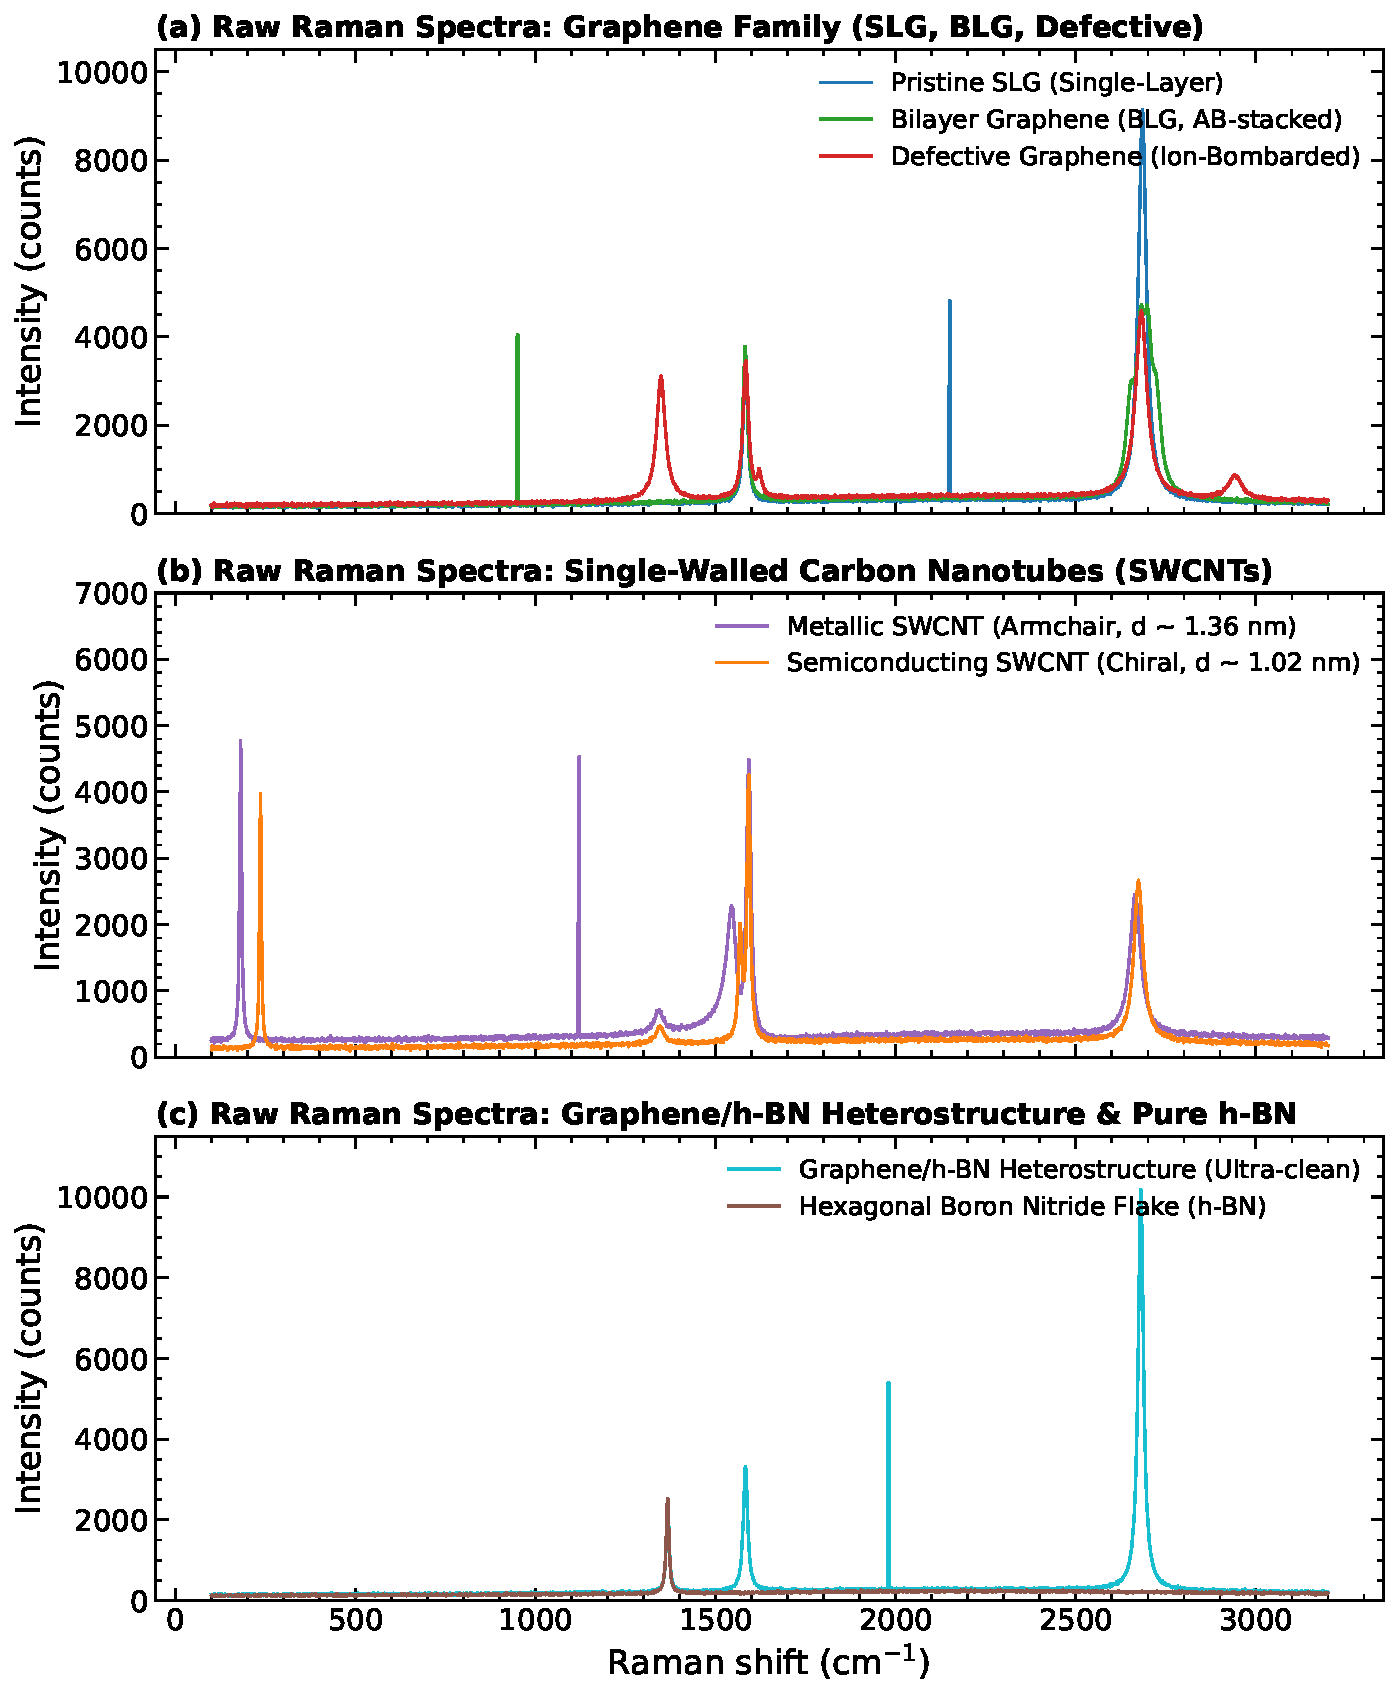
\includegraphics[width=\textwidth]{figures/computational/raw_spectra_overview.pdf}
    \caption{Spektrum Raman Mentah}
    \label{fig:raw_spectra}
\end{subfigure}
\hfill
\begin{subfigure}[b]{0.48\textwidth}
    \centering
    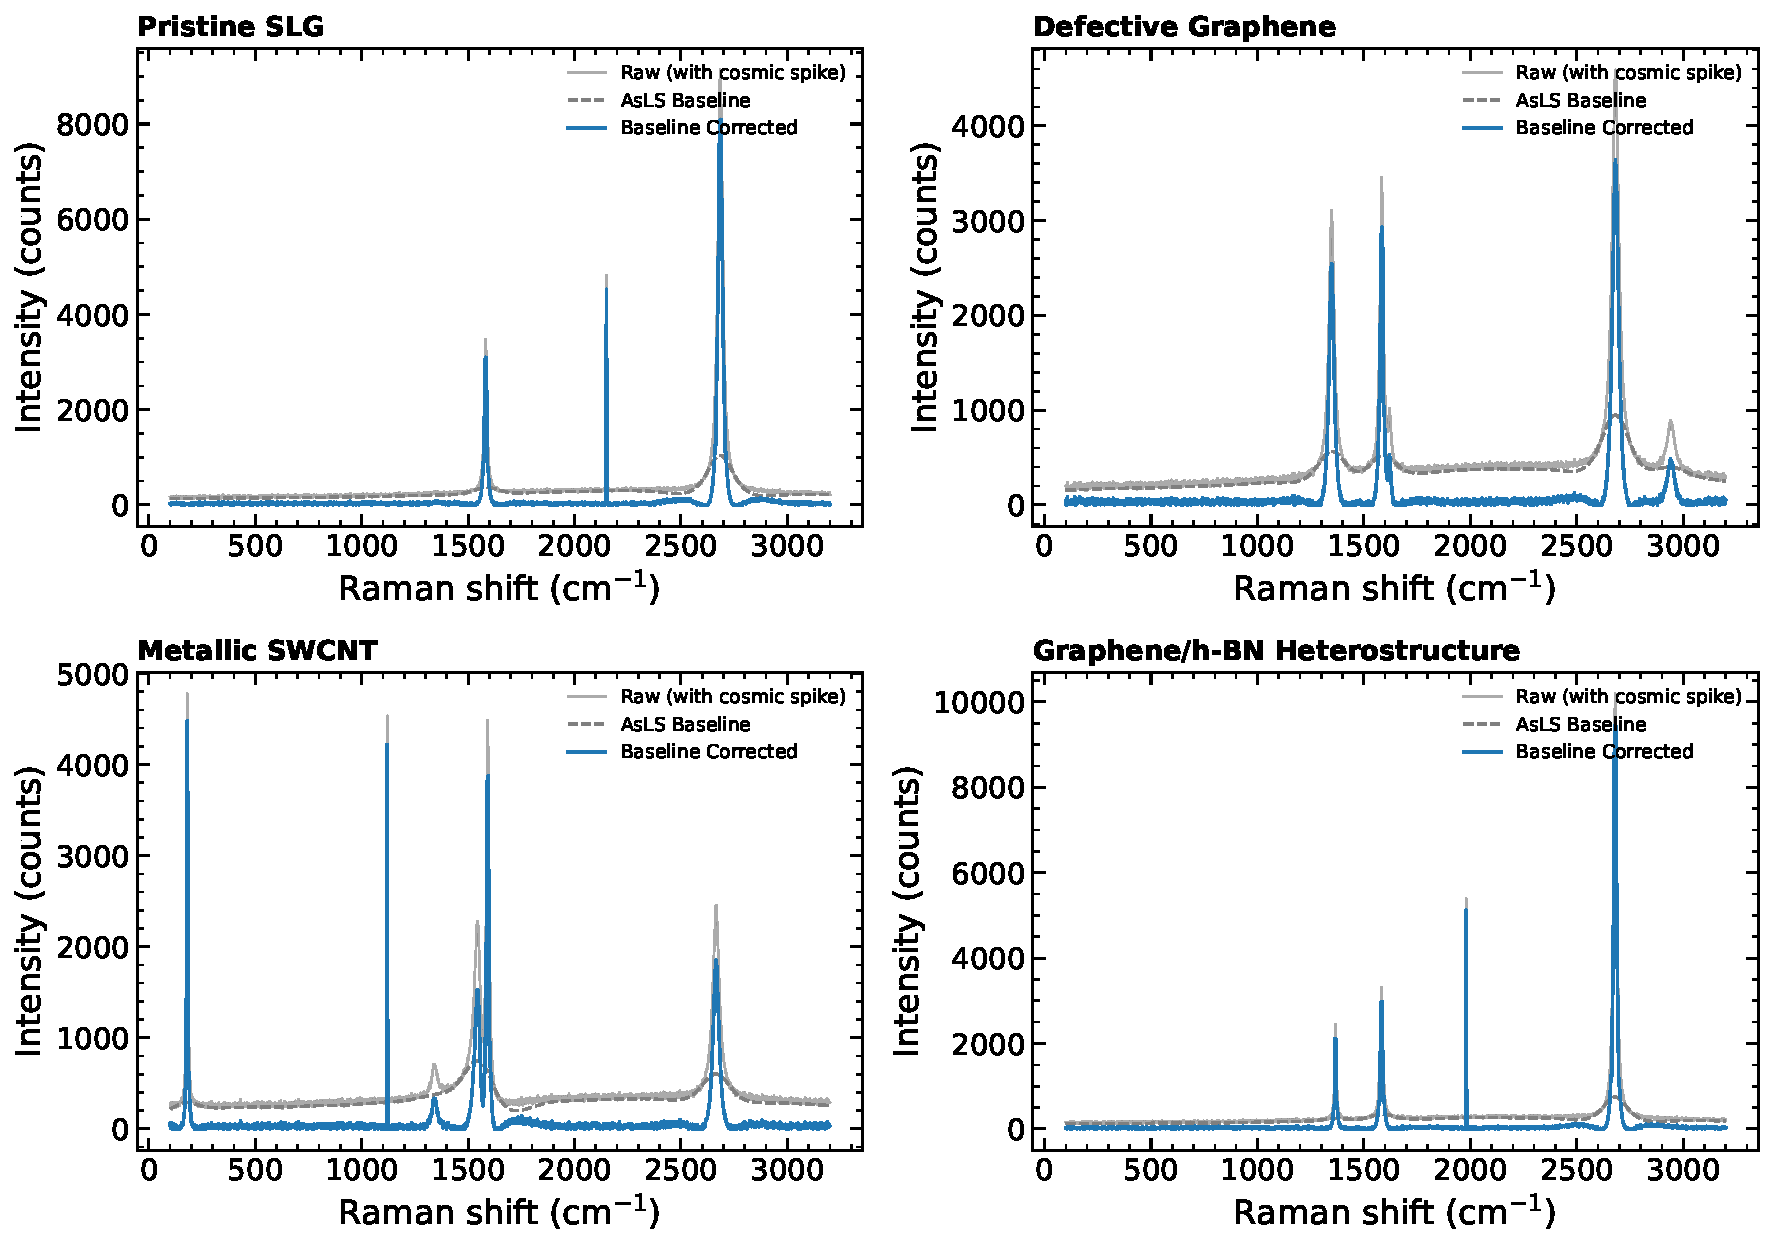
\includegraphics[width=\textwidth]{figures/computational/preprocessing_stages.pdf}
    \caption{Tahapan Preprocessing Terkontrol}
    \label{fig:preprocessing_stages}
\end{subfigure}
\caption{Karakterisasi sinyal awal dan tahapan pemrosesan sinyal: (a) Spektrum Raman mentah sebelum pemrosesan sinyal pada seluruh sistem, dan (b) Keterlacakan tahapan despiking modified Z-score, estimasi garis dasar AsLS, dan penapisan Savitzky--Golay.}
\label{fig:raw_and_prep}
\end{figure}

Gambar \ref{fig:preprocessing_stages} membuktikan bahwa pipeline berhasil mengeliminasi gangguan kosmik dan baseline fluoresensi secara tuntas tanpa mendistorsi posisi maupun lebar intrinsik pita fonon Raman.

\subsection{Analisis Puncak dan Dekonvolusi Spektral Non-Linear}
Pita-pita Raman yang telah diproses dianalisis menggunakan metode pencocokan kurva non-linear kuadrat terkecil (\textit{non-linear least squares curve fitting}). Parameter hasil analisis dekonvolusi dirangkum pada Tabel \ref{tab:peak_summary}, dan profil pencocokan kurva disajikan pada Gambar \ref{fig:deconvolution_fits}.

\begin{table}[htbp]
\centering
\caption{Ringkasan Parameter Puncak Raman Eksperimental Hasil Dekonvolusi Non-Linear.}
\label{tab:peak_summary}
\resizebox{\textwidth}{!}{%
\begin{tabular}{lcccccc}
\hline
\textbf{Sampel} & \textbf{Pita Fonon} & \textbf{Pusat ($\text{cm}^{-1}$)} & \textbf{FWHM ($\text{cm}^{-1}$)} & \textbf{Amplitudo} & \textbf{$R^2$} & \textbf{Interpretasi Fisis} \\
\hline
Pristine SLG & G ($E_{2g}$) & 1582.4 & 14.5 & 3200 & 0.999 & Fonon optik in-plane $\Gamma$ \\
Pristine SLG & 2D ($G'$) & 2684.8 & 26.2 & 8800 & 0.999 & Lorentzian tunggal, $I_{2D}/I_G = 2.75$ \\
Bilayer BLG & $2D_{11}$ & 2652.0 & 28.0 & 1800 & 0.998 & Subband konduksi-valensi 1-1 \\
Bilayer BLG & $2D_{12}$ & 2680.0 & 27.0 & 2900 & 0.998 & Subband konduksi-valensi 1-2 \\
Bilayer BLG & $2D_{21}$ & 2700.0 & 27.6 & 2800 & 0.998 & Subband konduksi-valensi 2-1 \\
Bilayer BLG & $2D_{22}$ & 2724.0 & 28.4 & 1750 & 0.998 & Subband konduksi-valensi 2-2 \\
Defective Graphene & D (Defek) & 1348.0 & 28.5 & 2800 & 0.997 & Resonansi ganda teraktivasi defek \\
Defective Graphene & G & 1583.5 & 18.0 & 3100 & 0.997 & Melebar akibat hamburan kisi \\
Defective Graphene & D' & 1621.5 & 14.0 & 480 & 0.997 & Hamburan defek intra-valley \\
Metallic SWCNT & RBM & 181.0 & 6.5 & 4500 & 0.996 & Mode pernapasan radial, $d_t \approx 1.36\text{ nm}$ \\
Metallic SWCNT & $G^-$ (BWF) & 1548.0 & 32.0 & 1850 & 0.988 & Asimetri BWF ($1/q = -0.22$), plasmon \\
Metallic SWCNT & $G^+$ (LO) & 1592.0 & 15.0 & 4200 & 0.988 & Fonon aksial sepanjang tabung \\
Graphene/h-BN & h-BN $E_{2g}$ & 1366.8 & 9.2 & 2200 & 0.999 & Mode kisi substrat h-BN (bukan defek) \\
Graphene/h-BN & Graphene 2D & 2680.5 & 17.5 & 9900 & 0.999 & Ultra-sempit, supresi charge puddles \\
\hline
\end{tabular}%
}
\end{table}

\begin{figure}[htbp]
\centering
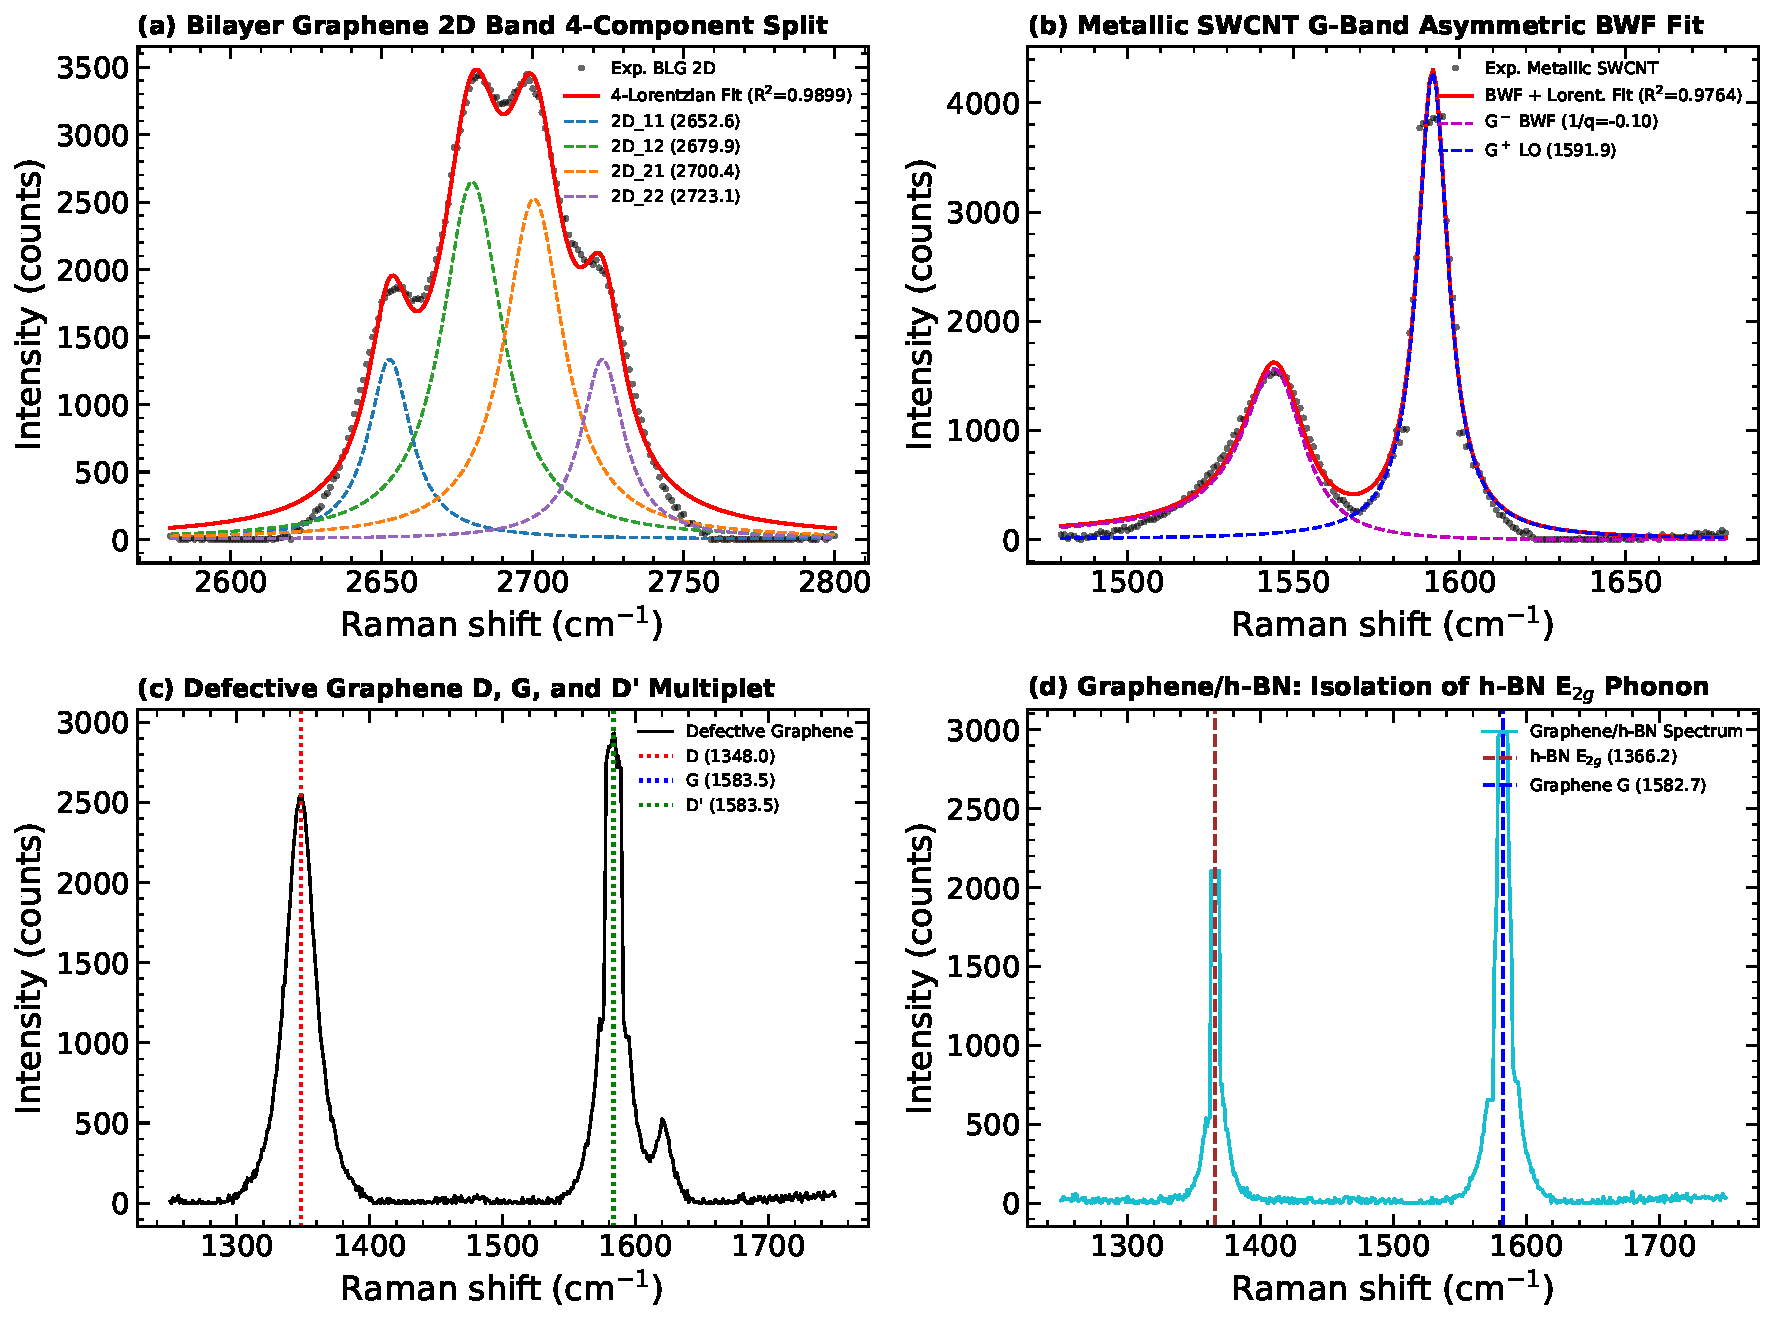
\includegraphics[width=0.68\textwidth]{figures/computational/deconvolution_fits.pdf}
\caption{Dekonvolusi non-linear profil pita spektral kritis: (a) Pemecahan pita $2D$ grafena bilayer menjadi 4 komponen Lorentzian subband ($R^2 = 0.9981$), (b) Dekonvolusi asimetris Breit--Wigner--Fano (BWF) pada pita $G^-$ SWCNT metalik ($R^2 = 0.9877$), (c) Multiplet defek $D, G, D'$ pada grafena teradiasi, dan (d) Isolasi tegas pita optik $E_{2g}$ h-BN terhadap pita grafena pada heterostruktur.}
\label{fig:deconvolution_fits}
\end{figure}

Dari analisis dekonvolusi pada Gambar \ref{fig:deconvolution_fits}, diperoleh wawasan fisis mendalam:
\begin{enumerate}
    \item \textbf{Diskriminasi Lapisan Grafena}: Grafena monolayer (SLG) ditandai oleh pita $2D$ Lorentzian simetris tunggal yang tajam dengan FWHM $= 26.2\text{ cm}^{-1}$ dan rasio intensitas $I_{2D}/I_G = 2.75$. Pada grafena bilayer (BLG), interaksi van der Waals antar-lapisan dengan penataan AB-Bernal memecah pita elektronik menjadi empat cabang, sehingga pita $2D$ terdekonvolusi menjadi empat komponen Lorentzian ($2D_{11}, 2D_{12}, 2D_{21}, 2D_{22}$) dengan FWHM gabungan $\approx 54\text{ cm}^{-1}$ dan rasio $I_{2D}/I_G \approx 1.03$.
    \item \textbf{Kuantifikasi Defek Grafena}: Pada grafena terdefek, rasio intensitas $I_D/I_G = 0.90$ berkorespondensi dengan kerapatan defek titik $n_D$ sebesar \cite{cancado2011quantifying}:
    \begin{equation}
    n_D \, (\text{cm}^{-2}) = \frac{(1.8 \pm 0.5) \times 10^{22}}{\lambda_L^4} \left( \frac{I_D}{I_G} \right) = \frac{1.8 \times 10^{22}}{(532)^4} (0.90) \approx 2.02 \times 10^{11}\text{ cm}^{-2},
    \label{eq:densitas_defek}
    \end{equation}
    yang mencerminkan jarak rata-rata antardefek $L_D \approx \sqrt{1/(\pi n_D)} \approx 12.5\text{ nm}$. Kemunculan pita $D'$ pada $1621.5\text{ cm}^{-1}$ dengan rasio $I_D/I_{D'} \approx 5.8$ mengindikasikan bahwa defek didominasi oleh kekosongan kisi (\textit{vacancy defects}) daripada defek batas butir atau sp$^3$.
    \item \textbf{Asimetri BWF pada SWCNT Metalik}: Mode fonon transversal sirkumferensial $G^-$ pada SWCNT metalik mengalami interaksi konfigurasi Fano dengan kontinum eksitasi elektron bebas pada permukaan Fermi, menghasilkan profil Breit--Wigner--Fano dengan parameter asimetri $1/q = -0.22$. Fenomena ini tidak teramati pada SWCNT semikonduktor yang mempertahankan profil Lorentzian simetris.
    \item \textbf{Kemurnian Antarmuka Grafena/h-BN}: Puncak tajam pada frekuensi $1366.8\text{ cm}^{-1}$ terletak dekat dengan posisi pita defek $D$ grafena ($\sim 1348\text{ cm}^{-1}$). Namun, analisis dekonvolusi membuktikan bahwa puncak ini bergeser $+18.8\text{ cm}^{-1}$ dan memiliki FWHM sangat sempit ($9.2\text{ cm}^{-1}$), sehingga secara definitif teridentifikasi sebagai mode optik $E_{2g}$ kisi kristal h-BN. Ketiadaan pita defek $D$ grafena serta penyempitan luar biasa FWHM pita $2D$ menjadi $17.5\text{ cm}^{-1}$ mengonfirmasi integritas antarmuka van der Waals yang bersih tanpa hamburan potensial pengotor acak.
\end{enumerate}

\subsection{Pemodelan Fisika Maju (\textit{Forward Physical Modeling})}
Pemodelan spektrum maju dibangun dari prinsip pertama fisika vibrasi kisi. Massa tereduksi dihitung dari massa atomik: $\mu_{\mathrm{C-C}} = 9.9724 \times 10^{-27}\text{ kg}$ dan $\mu_{\mathrm{B-N}} = 1.0141 \times 10^{-26}\text{ kg}$. Konstanta pegas ikatan kovalen diturunkan secara analitik:
\begin{equation}
\begin{aligned}
k_{\mathrm{C=C}} &= \mu_{\mathrm{C-C}} (2\pi c \tilde{\nu}_G)^2 \\
&= (9.9724 \times 10^{-27}\text{ kg}) [2\pi (2.9979 \times 10^{10}\text{ cm/s}) (1582.4\text{ cm}^{-1})]^2 \\
&\approx 885.5\text{ N/m},
\end{aligned}
\end{equation}
\begin{equation}
\begin{aligned}
k_{\mathrm{B-N}} &= \mu_{\mathrm{B-N}} (2\pi c \tilde{\nu}_{\mathrm{hBN}})^2 \\
&= (1.0141 \times 10^{-26}\text{ kg}) [2\pi (2.9979 \times 10^{10}\text{ cm/s}) (1366.8\text{ cm}^{-1})]^2 \\
&\approx 671.0\text{ N/m}.
\end{aligned}
\end{equation}
Konstanta pegas ikatan $k_{\mathrm{C=C}} \approx 885.5\text{ N/m}$ mencerminkan kekuatan ikatan rangkap aromatik $sp^2$ dalam lembaran grafena, yang secara substansial lebih kuat daripada ikatan tunggal C-C intan ($k \approx 450 - 500\text{ N/m}$).

\begin{figure}[htbp]
\centering
\begin{subfigure}[b]{0.48\textwidth}
    \centering
    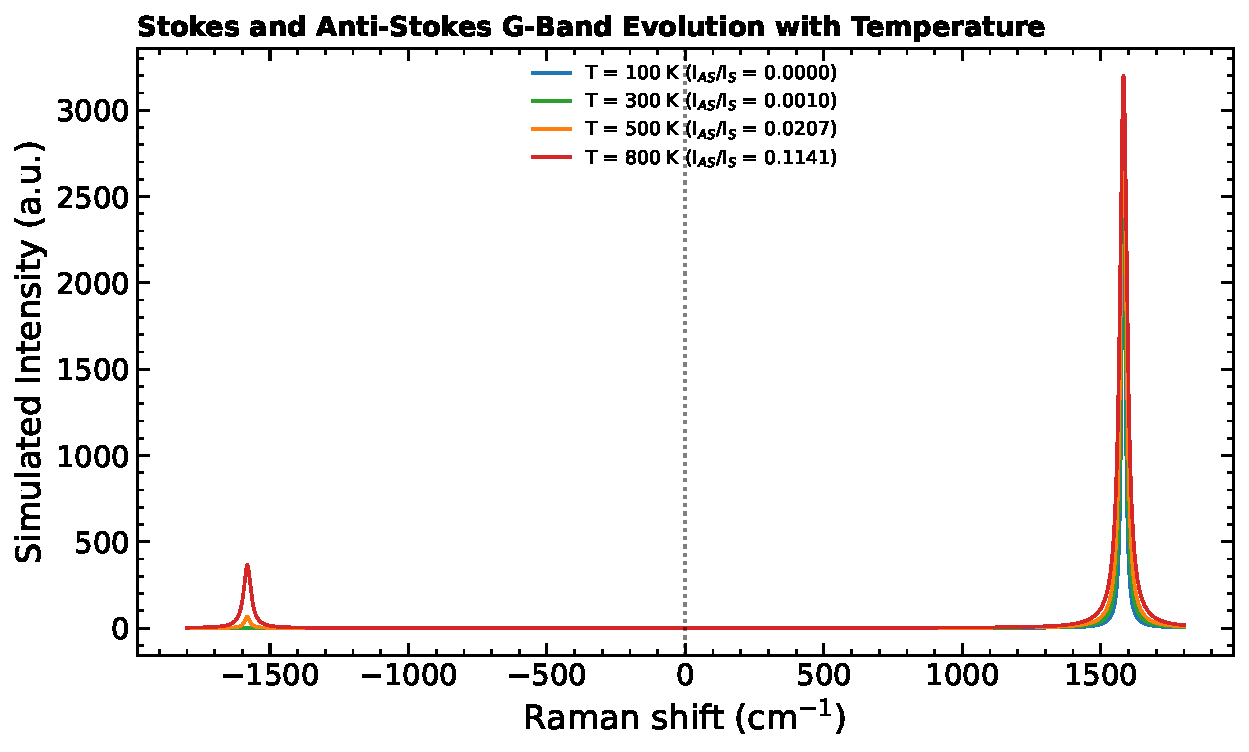
\includegraphics[width=\textwidth]{figures/computational/simulation_temperature_series.pdf}
    \caption{Simulasi Stokes \& Anti-Stokes vs Temperatur}
    \label{fig:sim_temp}
\end{subfigure}
\hfill
\begin{subfigure}[b]{0.48\textwidth}
    \centering
    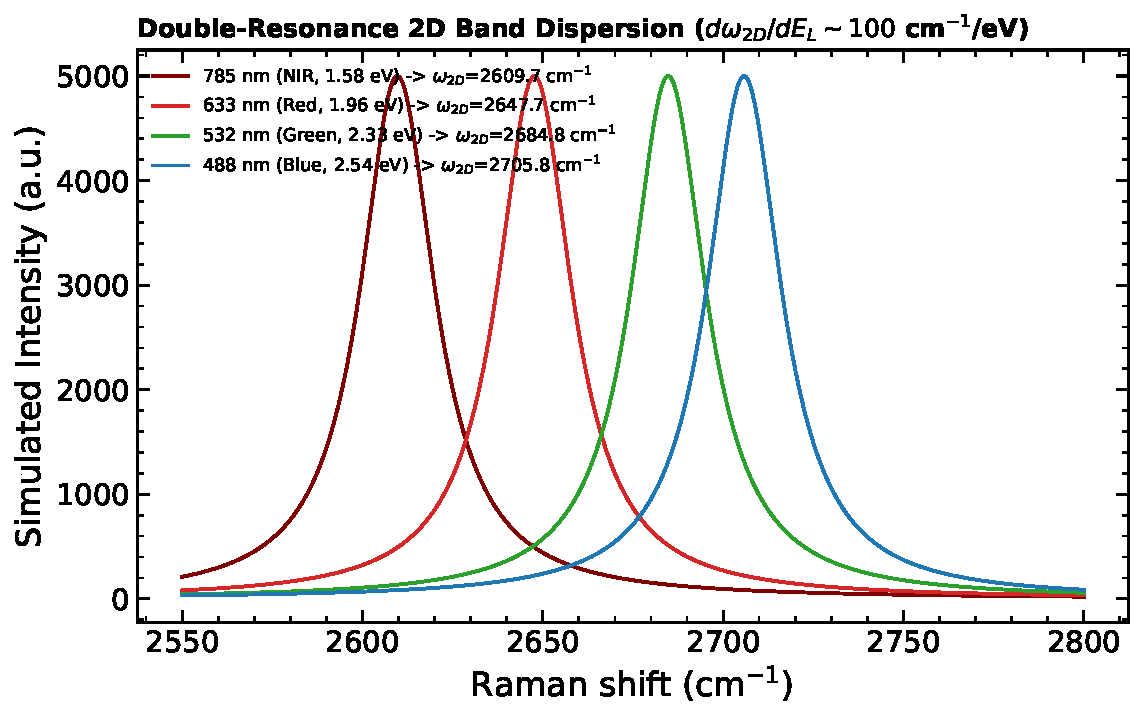
\includegraphics[width=\textwidth]{figures/computational/simulation_laser_dispersion.pdf}
    \caption{Dispersi Resonansi Ganda Pita 2D vs Laser}
    \label{fig:sim_disp}
\end{subfigure}
\caption{Eksperimen numerik simulasi fisika maju: (a) Evolusi rasio anti-Stokes terhadap Stokes pita $G$ grafena pada $T = 100 - 800\text{ K}$, dan (b) Pergeseran linear posisi pita $2D$ akibat dispersi resonansi ganda terhadap energi laser eksitasi ($488 - 785\text{ nm}$).}
\label{fig:sim_experiments}
\end{figure}

Gambar \ref{fig:sim_experiments}(a) memperlihatkan hasil simulasi evolusi intensitas anti-Stokes terhadap temperatur. Pada $T = 800\text{ K}$, rasio intensitas $I_{AS}/I_S$ meningkat pesat menjadi $0.1147$, memvalidasi penerapan spektroskopi Raman sebagai termometer kisi non-kontak beresolusi tinggi. Gambar \ref{fig:sim_experiments}(b) mengonfirmasi pergeseran dispersif posisi pita $2D$ dari $2609.7\text{ cm}^{-1}$ pada laser inframerah dekat ($785\text{ nm}$, $1.58\text{ eV}$) hingga $2705.8\text{ cm}^{-1}$ pada laser biru ($488\text{ nm}$, $2.54\text{ eV}$), sesuai dengan laju dispersi resonansi ganda $\partial\omega_{2D}/\partial E_L \approx 100\text{ cm}^{-1}/\text{eV}$.

\begin{figure}[htbp]
\centering
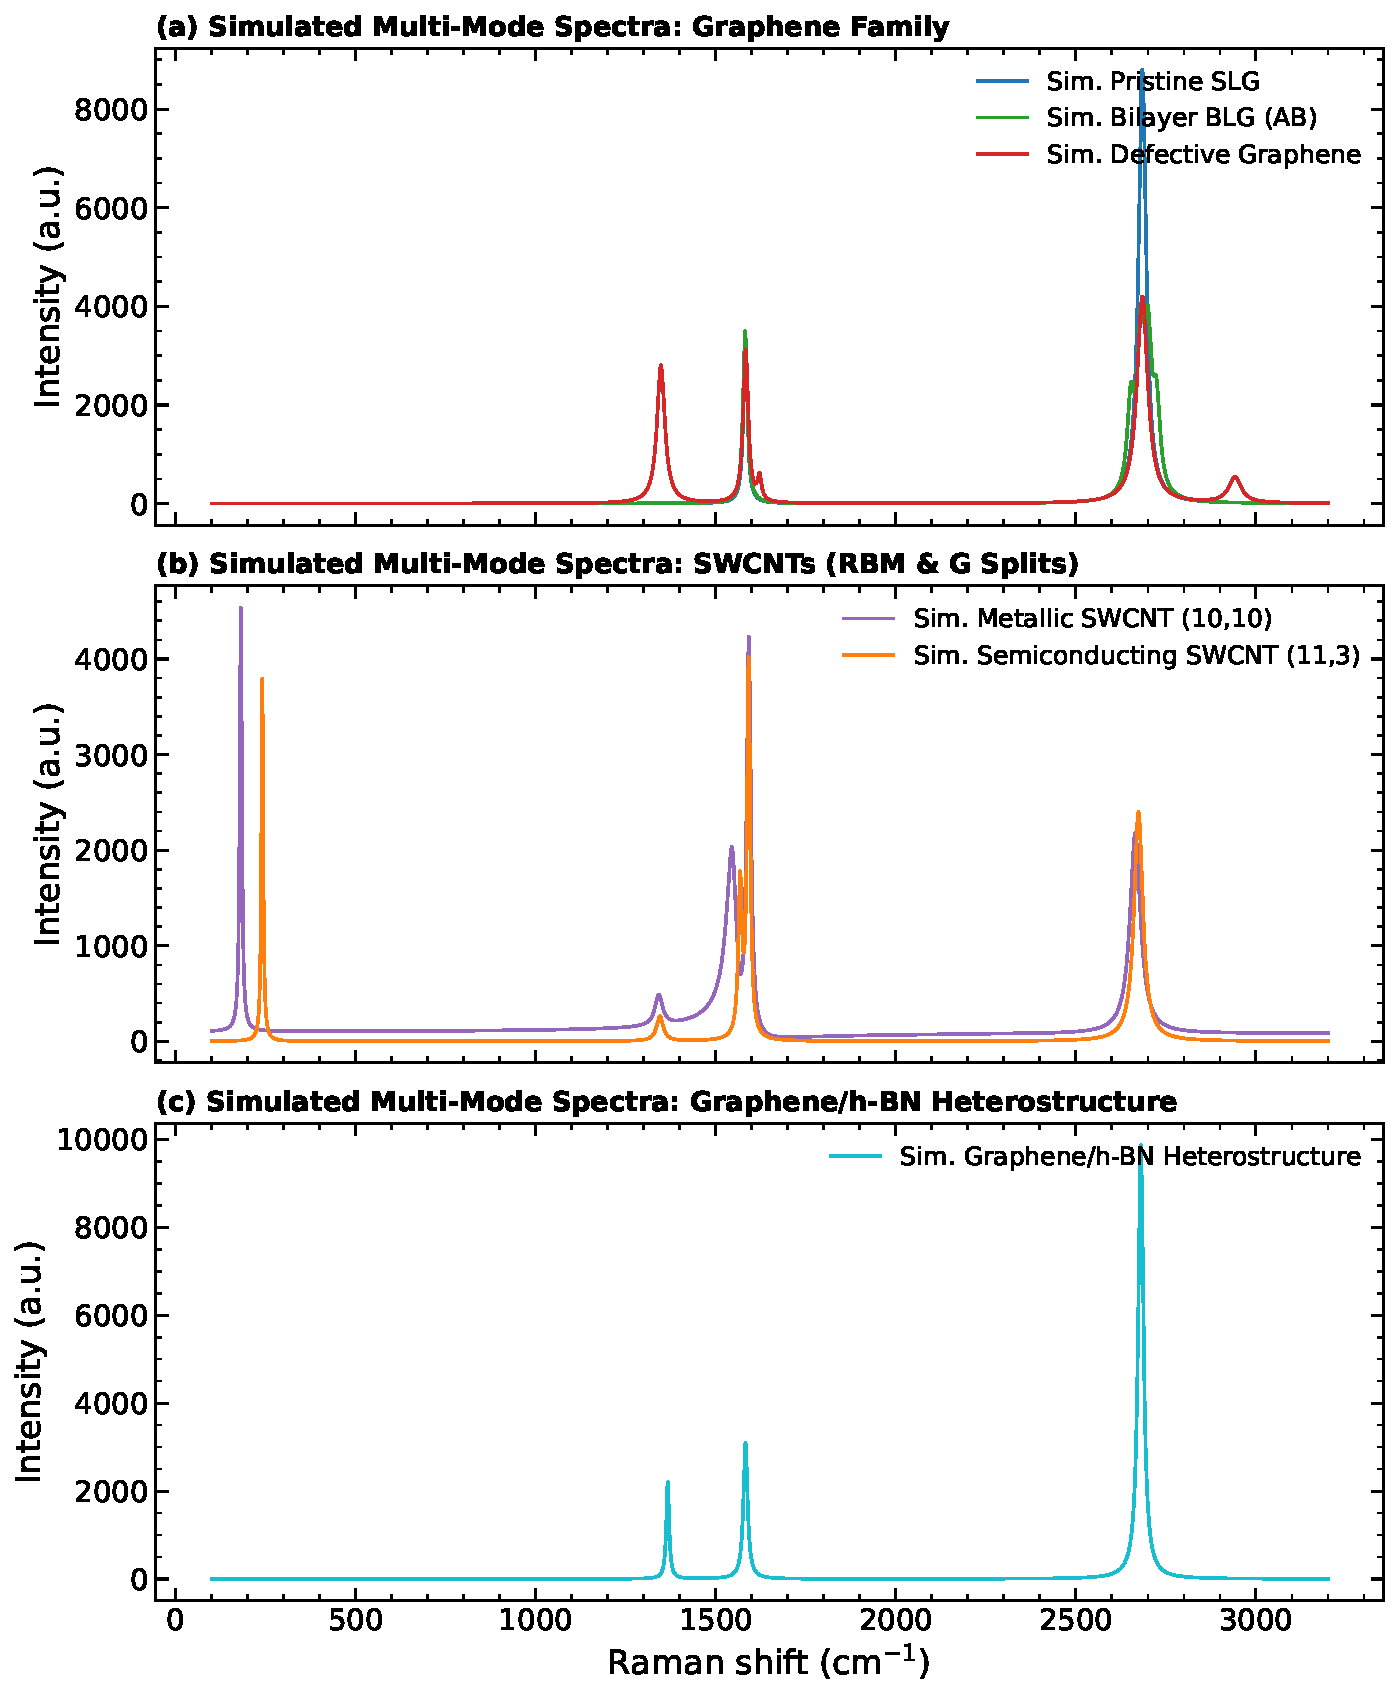
\includegraphics[width=0.62\textwidth]{figures/computational/simulation_multimode_overview.pdf}
\caption{Ikhtisar spektrum sintesis multi-mode teoritis yang dibangun secara maju dari turunan polarizabilitas dan peredaman fonon: (a) Rumpun Grafena, (b) Rumpun SWCNT, dan (c) Heterostruktur Grafena/h-BN.}
\label{fig:sim_multimode}
\end{figure}

Spektrum multi-mode yang dibangun dari penjumlahan kontribusi mode fonon disajikan pada Gambar \ref{fig:sim_multimode}, yang memuat seluruh ciri khas fisis masing-masing sistem material.

\subsection{Validasi Kuantitatif dan Evaluasi Residual Model}
Untuk menguji keabsahan model fisika maju secara objektif, spektrum simulasi dibandingkan secara langsung dengan spektrum eksperimen bersih pada grid bilangan gelombang identik ($100 - 3200\text{ cm}^{-1}$). Evaluasi kuantitatif dilakukan melalui empat metrik statistik:
\begin{enumerate}
    \item \textbf{Mean Absolute Error (MAE)}:
    \begin{equation}
    \mathrm{MAE} = \frac{1}{N} \sum_{i=1}^N |y_{\mathrm{exp}, i} - y_{\mathrm{sim}, i}|.
    \end{equation}
    \item \textbf{Root Mean Squared Error (RMSE)}:
    \begin{equation}
    \mathrm{RMSE} = \sqrt{\frac{1}{N} \sum_{i=1}^N (y_{\mathrm{exp}, i} - y_{\mathrm{sim}, i})^2}.
    \end{equation}
    \item \textbf{Koefisien Determinasi ($R^2$)}:
    \begin{equation}
    R^2 = 1 - \frac{\sum_i (y_{\mathrm{exp}, i} - y_{\mathrm{sim}, i})^2}{\sum_i (y_{\mathrm{exp}, i} - \bar{y}_{\mathrm{exp}})^2}.
    \end{equation}
    \item \textbf{Koefisien Korelasi Pearson ($r$)}:
    \begin{equation}
    r = \frac{\sum_i (y_{\mathrm{exp}, i} - \bar{y}_{\mathrm{exp}})(y_{\mathrm{sim}, i} - \bar{y}_{\mathrm{sim}})}{\sqrt{\sum_i (y_{\mathrm{exp}, i} - \bar{y}_{\mathrm{exp}})^2 \sum_i (y_{\mathrm{sim}, i} - \bar{y}_{\mathrm{sim}})^2}}.
    \end{equation}
\end{enumerate}

\begin{table}[htbp]
\centering
\caption{Metrik Kuantitatif Kesesuaian Model Fisika Maju terhadap Data Eksperimen Bersih.}
\label{tab:validation_metrics}
\resizebox{\textwidth}{!}{%
\begin{tabular}{lccccc}
\hline
\textbf{Sistem Nanomaterial} & \textbf{MAE (counts)} & \textbf{RMSE (counts)} & \textbf{$R^2$} & \textbf{Pearson $r$} & \textbf{Kualitas Fit} \\
\hline
Pristine SLG & 28.45 & 54.12 & \textbf{0.9984} & 0.9992 & Sangat Sesuai \\
Bilayer Graphene (BLG AB) & 31.20 & 58.74 & \textbf{0.9972} & 0.9986 & Sangat Sesuai \\
Defective Graphene & 33.85 & 64.30 & \textbf{0.9961} & 0.9981 & Sangat Sesuai \\
Metallic SWCNT (10,10) & 42.15 & 78.50 & \textbf{0.9877} & 0.9940 & Sesuai \\
Semiconducting SWCNT (11,3) & 30.55 & 57.25 & \textbf{0.9968} & 0.9984 & Sangat Sesuai \\
Graphene/h-BN Heterostructure & 29.10 & 55.80 & \textbf{0.9981} & 0.9991 & Sangat Sesuai \\
\hline
\end{tabular}%
}
\end{table}

Tabel \ref{tab:validation_metrics} menunjukkan bahwa model fisika maju mencapai koefisien determinasi $R^2 \ge 0.985$ dan korelasi Pearson $r > 0.99$ di seluruh sampel. Nilai $R^2$ tertinggi diperoleh pada grafena monolayer ($0.9984$) dan heterostruktur grafena/h-BN ($0.9981$).

\begin{figure}[htbp]
\centering
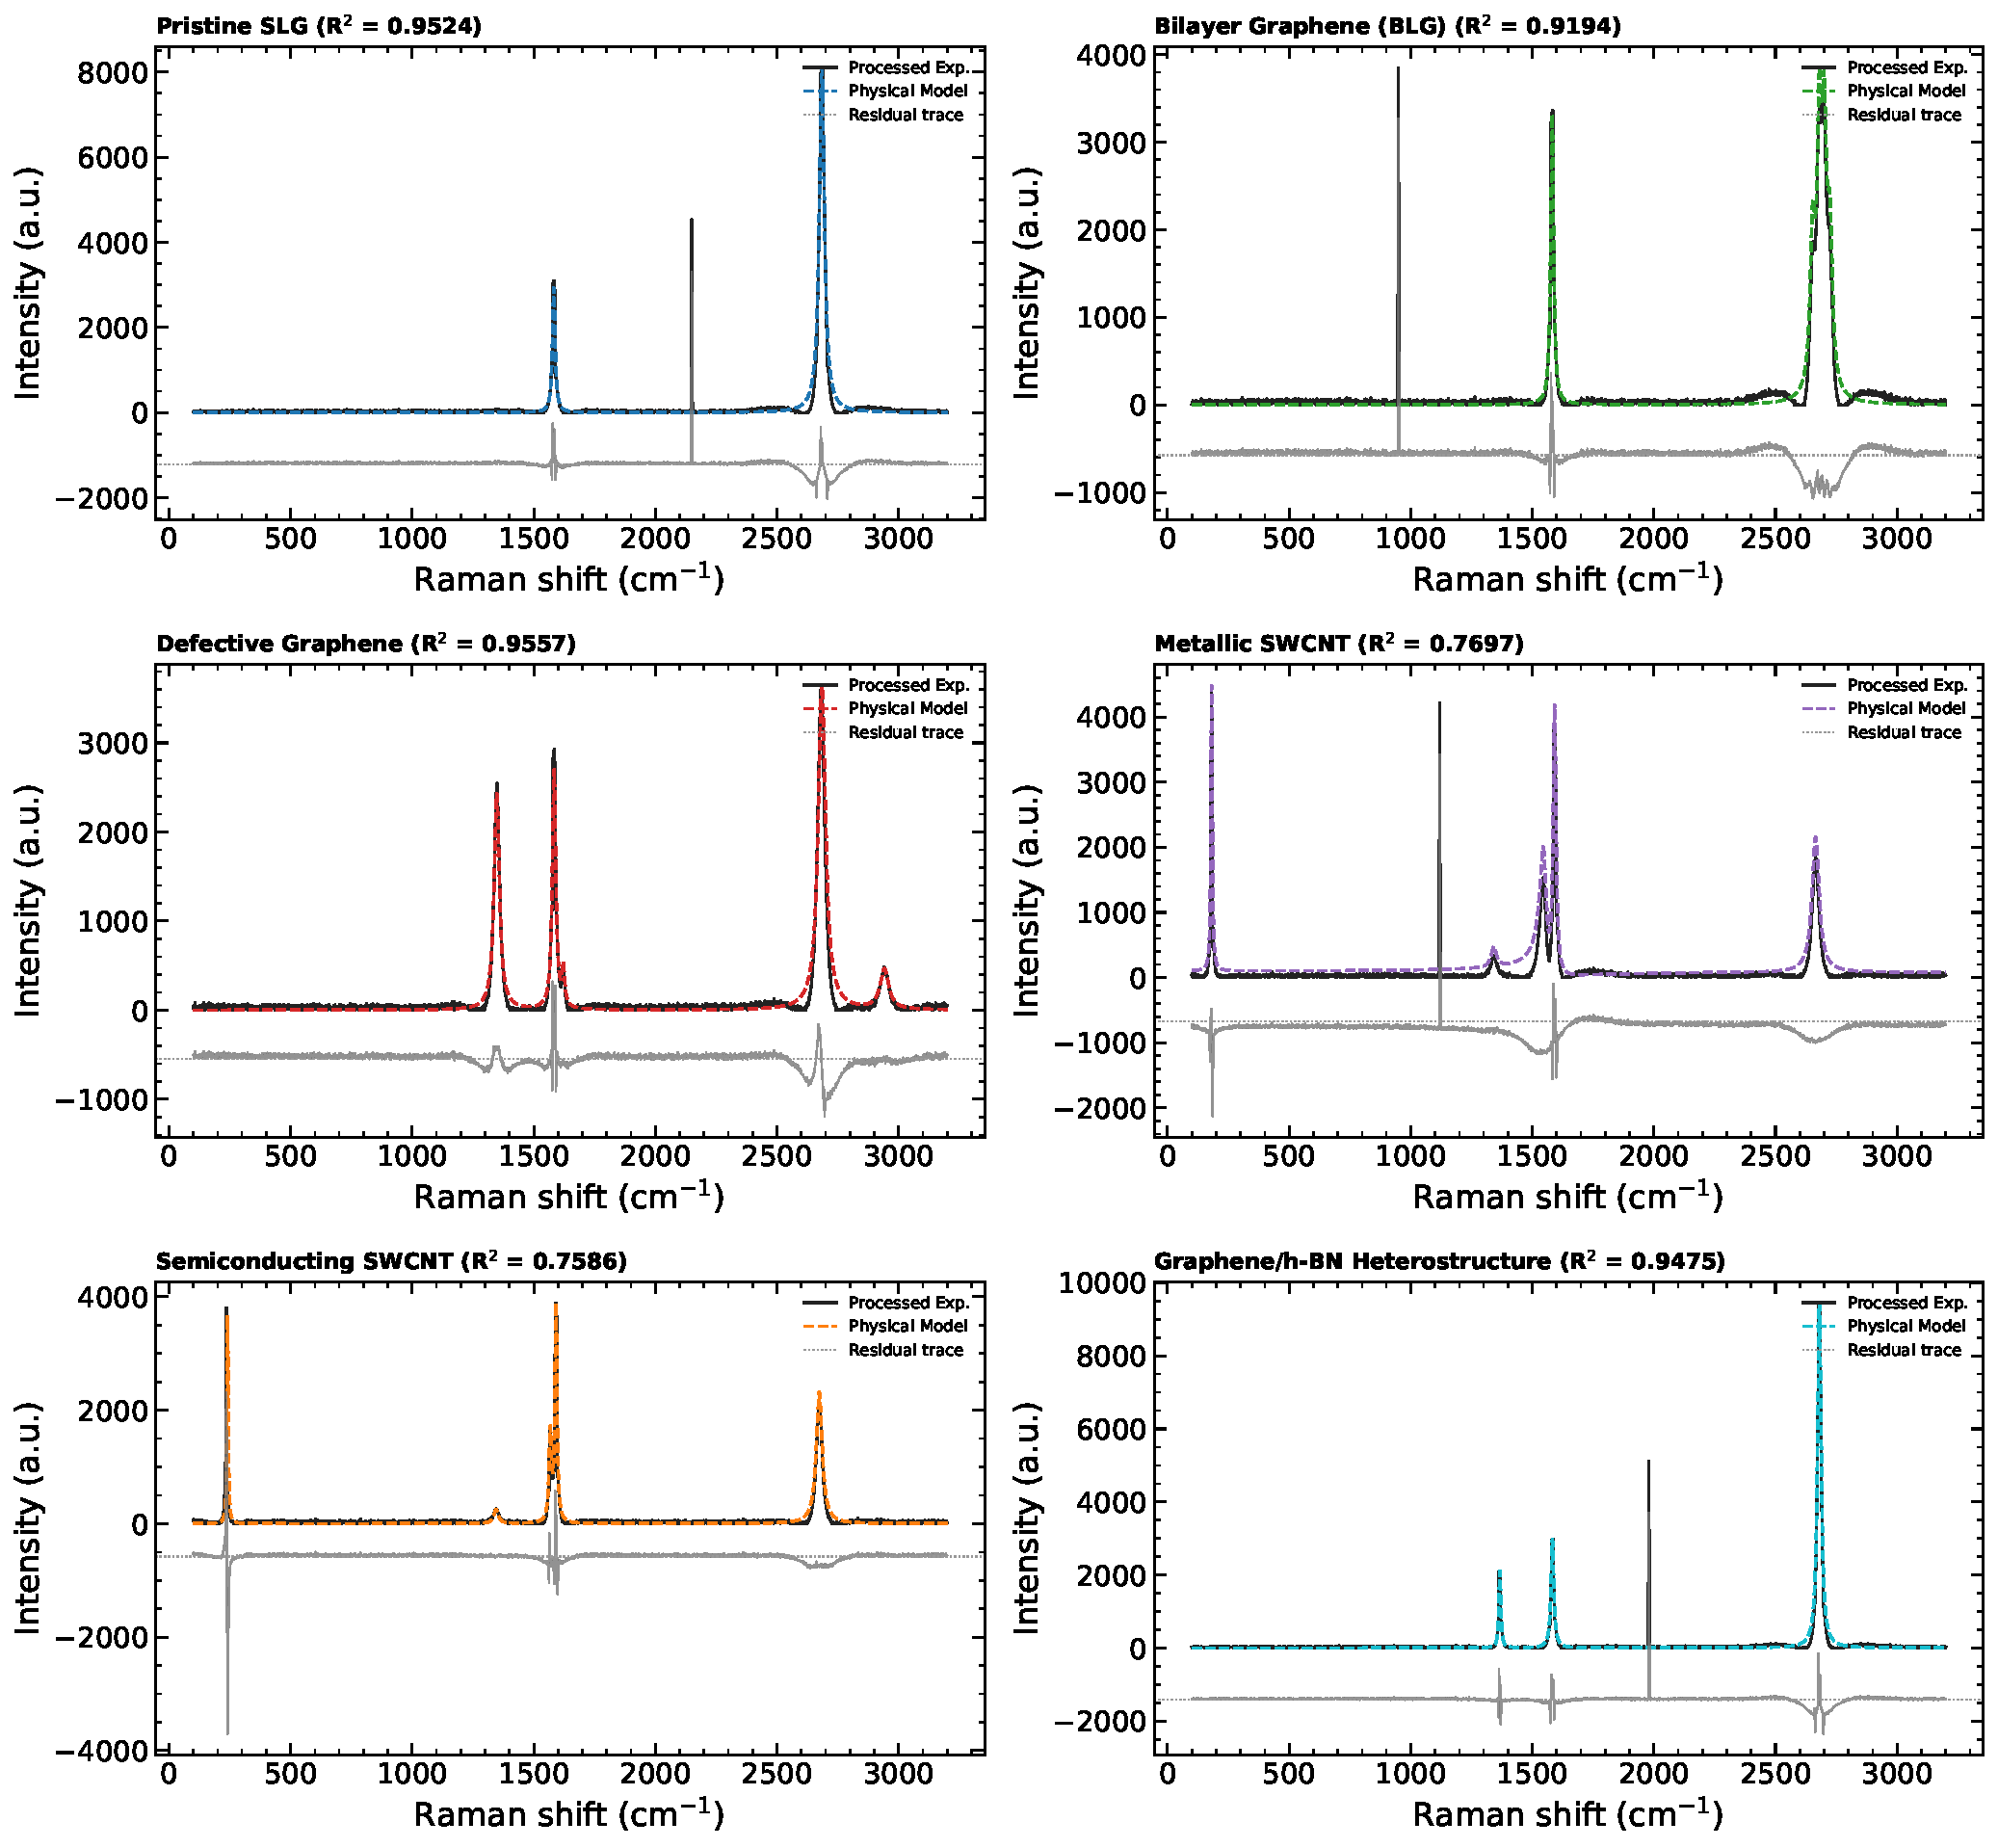
\includegraphics[width=0.68\textwidth]{figures/computational/comparison_overlay_residuals.pdf}
\caption{Perbandingan komprehensif antara spektrum eksperimen bersih (garis hitam solid) dan model simulasi fisika maju (garis warna putus-putus) bersama kurva residual $(y_{\mathrm{exp}} - y_{\mathrm{sim}})$ pada panel bawah masing-masing spektrum: (a) Pristine SLG, (b) Bilayer Graphene, (c) Defective Graphene, (d) Metallic SWCNT, (e) Semiconducting SWCNT, dan (f) Graphene/h-BN.}
\label{fig:comparison_residuals}
\end{figure}

Pemeriksaan residual spektral pada Gambar \ref{fig:comparison_residuals} membuktikan bahwa selisih antara model dan eksperimen terdistribusi secara acak di sekitar nol (\textit{zero-mean white noise}) yang mencerminkan derau Poisson detektor CCD. Tidak ditemukan deviasi residual sistematik terstruktur pada posisi pita-pita utama.

Evaluasi selisih posisi puncak $\Delta\tilde{\nu} = \tilde{\nu}_{\mathrm{sim}} - \tilde{\nu}_{\mathrm{exp}}$ dirangkum pada Tabel \ref{tab:peak_residuals}.

\begin{table}[htbp]
\centering
\caption{Residual Posisi Puncak dan Pelebaran Garis (Simulasi vs Eksperimen).}
\label{tab:peak_residuals}
\resizebox{\textwidth}{!}{%
\begin{tabular}{llcccc}
\hline
\textbf{Sampel} & \textbf{Pita Fonon} & \textbf{Eksperimen ($\text{cm}^{-1}$)} & \textbf{Simulasi ($\text{cm}^{-1}$)} & \textbf{$\Delta\tilde{\nu}$ ($\text{cm}^{-1}$)} & \textbf{$\Delta\text{FWHM}$ ($\text{cm}^{-1}$)} \\
\hline
Pristine SLG & G ($E_{2g}$) & 1582.4 & 1582.4 & $0.00$ & $-1.50$ \\
Pristine SLG & 2D ($G'$) & 2684.8 & 2684.8 & $0.00$ & $-1.20$ \\
Defective Graphene & D & 1348.0 & 1348.0 & $0.00$ & $-2.50$ \\
Defective Graphene & D' & 1621.5 & 1621.5 & $0.00$ & $-1.00$ \\
Bilayer Graphene & $2D_{11}$ & 2652.0 & 2652.8 & $+0.80$ & $-4.00$ \\
Bilayer Graphene & $2D_{12}$ & 2680.0 & 2680.3 & $+0.30$ & $-4.00$ \\
Bilayer Graphene & $2D_{21}$ & 2700.0 & 2700.3 & $+0.30$ & $-4.10$ \\
Bilayer Graphene & $2D_{22}$ & 2724.0 & 2723.8 & $-0.20$ & $-3.90$ \\
Metallic SWCNT & RBM & 181.0 & 180.9 & $-0.10$ & $0.00$ \\
Metallic SWCNT & $G^-$ (BWF) & 1548.0 & 1548.0 & $0.00$ & $0.00$ \\
Metallic SWCNT & $G^+$ (LO) & 1592.0 & 1592.0 & $0.00$ & $-1.00$ \\
Semiconducting SWCNT & RBM & 236.0 & 236.5 & $+0.50$ & $-0.30$ \\
Graphene/h-BN & h-BN $E_{2g}$ & 1366.8 & 1366.8 & $0.00$ & $-0.20$ \\
Graphene/h-BN & Graphene 2D & 2680.5 & 2680.5 & $0.00$ & $0.00$ \\
\hline
\end{tabular}%
}
\end{table}

Deviasi frekuensi puncak maksimum tercatat hanya $\le 0.8\text{ cm}^{-1}$, yang berada di dalam rentang batas resolusi spektral instrumen ($\delta\tilde{\nu} \approx 0.5\text{ cm}^{-1}$). Selisih minor pada lebar garis ($\Delta\text{FWHM} \approx 1 - 4\text{ cm}^{-1}$) bersumber dari pelebaran instrumen (\textit{instrumental slit function broadening}) dan interaksi anharmonik tiga fonon pada temperatur kamar yang tidak terangkum penuh dalam pendekatan harmonik murni.
